In questo capitolo verrà descritta la procedura di deployment dei componenti Wasm nella piattaforma wasmCloud. La comunicazione fra questa ed il framework PELATO avviene tramite NATS: sarà sufficiente configurare il framework con le credenziali di un client NATS collegato al cluster per poter deployare le applicazioni.\\
Anche in questo caso il componente deploy si appoggia a Docker per l'operazione, dato che l'applicazione del deployment tramite il manifest \texttt{wadm.yaml} ottenuto in fase di Generazione deve essere effettuata utilizzando \texttt{wash}.

\section{Application Deployment}

La fase di deployment è strutturata in modo molto simile a quella di build, infatti le operazioni svolte dal componente deploy sono:

\begin{enumerate}
    \item Istanziamento del client Docker.
    \item Controllo dell'immagine \texttt{wash-deploy-image:latest}, se non è presente procede a buildarla utilizzando il dockerfile configurato.
    \item Per ogni cartella presente dentro \texttt{gen} istanzia un container con \texttt{wash-deploy-image} come immagine e monta la cartella all'interno del container.
    \item Attende la terminazione dei container.
\end{enumerate}

\subsubsection{Wash deploy image}

 Il Dockerfile utilizzato per buildare l'immagine \texttt{wash-deploy-image} è più semplice, in quanto deve solamente installare la wasmCloud shell e le sue dipendenze:
 
\begin{lstlisting}[language=Dockerfile, caption={wash-build-image Dockerfile}, captionpos=b, label={code:wash_buil_image_dockerfile}, basicstyle=\ttfamily\small]
FROM ubuntu:24.04 AS wash-deploy-image

# Install dependencies and tools
RUN apt-get update && apt-get install -y curl wget tar ...

# ----------------- Install WasmCloud -----------------
RUN curl -s "https://packagecloud.io/install/repositories/wasmcloud/core/script.deb.sh" | bash && \
    apt-get install -y wash

# ----------------- Deploy the WasmCloud module -----------------
FROM wash-deploy-image

RUN mkdir /app
WORKDIR /app

# Deploy the WasmCloud module
CMD ["sh", "-c", "wash app deploy wadm.yaml"]
\end{lstlisting}

\subsection{Deployer}

Il comando riportato nell'istruzione CMD in questo caso è \texttt{wash app deploy wadm.yaml}, che utilizza il file wadm.yaml per creare un'applicazione sul cluster wasmCloud specificato.\\
L'approccio utilizzato per eseguire i processi di deployment è analogo a quello della fase Build, la differenza sta nelle variabili d'ambiente necessarie all'operazione: in questo caso sarà necessario fornire hostname e porta di un server NATS collegato al cluster wasmCloud. Di seguito viene riportata la porzione di codice che si occupa di eseguire il container.\\

\begin{lstlisting}[language=python, caption={Deploy applicazione su wasmCloud}, captionpos=b, label={code:deploy}]
def __deploy_wadm(task_dir, client, nats_host, nats_port, detached, wait_list):
    path = os.path.abspath(task_dir) + '/wadm.yaml'
    name = wadm['spec']['components'][0]['name'] + '-deploy'
    ...
    # Deploy wasmCloud app
    print(f" - Deploying WASM module {name}")
    container = client.containers.run(
        "wash-deploy-image:latest",
        environment=[f'WASMCLOUD_CTL_HOST={nats_host}',
                     f'WASMCLOUD_CTL_PORT={nats_port}'],
        volumes={path: {'bind': '/app/wadm.yaml', 'mode': 'rw'}},
        remove=True,
        detach=True,
        name=name
    )
    
    if detached == 'False':
        container.wait()
    else:
        wait_list.append(name)
\end{lstlisting}

\subsection{Remover}

Nel package \texttt{component\_deploy} è presente anche la funzionalità \texttt{remove}, con codice e comportamenti analoghi a quella di deploy. L'unica differenza si presenta nel dockerfile, nel quale l'istruzione specificata nel CMD è \texttt{wash app remove wadm.yaml} e permette di rimuovere le applicazioni specificate sui file wadm dal cluster.\\

\section{Processo completo}

Anche in questo caso è possibile parallelizzare l'esecuzione dei container, sia in fase di deployment che di rimozione delle applicazioni. L'intero processo di deployment viene mostrato nella Figura \ref{fig:impl_build}.

\FloatBarrier
\begin{figure}[h]
    \centering
    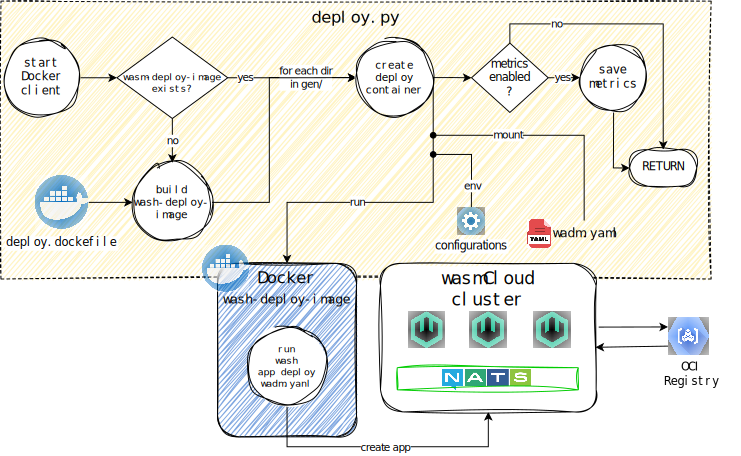
\includegraphics[width=\textwidth]{img/schemi/schemi-implementazione-deploy.drawio.pdf}
    \caption{Processo deployment applicazione su wasmCloud}
    \label{fig:impl_deploy}
\end{figure}
\FloatBarrier